\chapter{Constructing the Convolutional Neural Network }
This chapter will break down the process needed to build a convolutional neural network with PyTorch. The PyTorch library comes with a number of tutorials that work well on the large datasets that they provide in order to load the data in bulk and train your neural network using GPUs to parallelise the process. However, the data that most remote sensing scientists have is not in tiles with one land use class per tile, but rather in extremely large images with lots of varied land use across the field of view. This thesis aims to standardise the procedure using data more typical of remote sensing applications.
\paragraph{}
Convolutional Neural Networks or CNNs are similar to neural networks as they are made up of neurons with learnable weights and biases, just like random forests (RF) (\cite{belgiu16,Breiman01}) and support vector machine (SVM) (\cite{cortes95,mountrakis11,vapnik82}) learning. Each neuron has an input and output \textit{feature map}, where each \textit{feature map} represents a particular feature extracted from the input (\cite{lecun10}). A neuron in the case of our model is each kernel of data taken from the input image. For an image that is 256x256 pixels and with a moving kernel of 4x4 pixels, there would be 64 neurons in the output volume. 
\par 
Compared to regular neural networks, CNNs explicitly assume the inputs are images allowing certain properties to be encoded. Regular neural networks transform images through a series of hidden layers. Each layer is made up of neurons with each neuron connected to every neuron in the the previous layer but each neuron in one layer is not connect to any other neuron in the same layer (Figure \ref{fig.convolve_data})(\cite{karpathy_cnn1}). The last layer contains the class score for each pixel, indicating what class that pixel is most likely to belong to. 
\par 
Regular networks do not scale well to images that have multiple channels of information. For remote sensing, in most cases, the imagery will have at least three layers of information, if not more. In a regular network, an image that is 256x256 pix with three channels equates to 196,000 weights to calculate, for just one neuron (\cite{karpathy_cnn1}). In the example case above, there are 64 neurons resulting in over 12 million weights to calculate in the first layer. Large numbers of parameters results in the network memorising the training set by creating a function that matches the training set but does not generalise to unseen areas, i.e. overfitting (\cite{dietterich95}). CNNs take advantage of the 3D volume of neurons so each neuron has height, width and depth dimensions where the depth corresponds to the number of bands in the image (Figure \ref{fig.convolve_data}). Each neuron in each layer will only be connected to a small region of the previous layer, instead of all the neurons. This reduces the number of parameters and is why CNNs are different to regular neural networks (\cite{karpathy_cnn1}). For image classification where the image sizes are extremely large, CNNs are a better alternative to regular neural networks.
\begin{figure}[htbp]
    \centering
    %\begin{subfigure}{0.45\textwidth}
    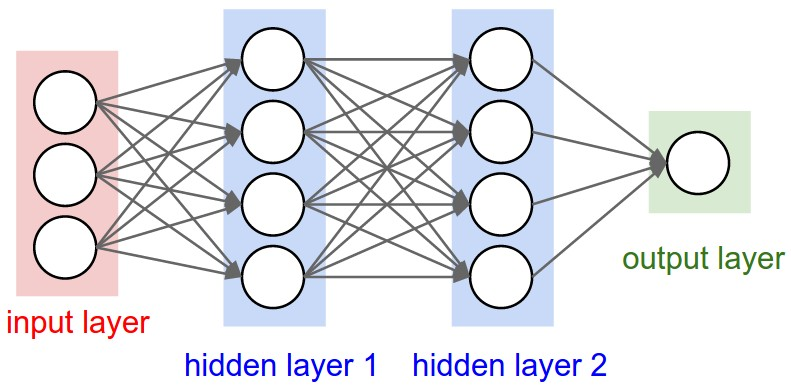
\includegraphics[width=0.5\textwidth]{\dir/figs/convolve_data.jpeg}
    %\caption{}
    %\label{fig.convolve_data1}
    %\end{subfigure}%
    %\qquad
    %\begin{subfigure}{0.45\textwidth}
    %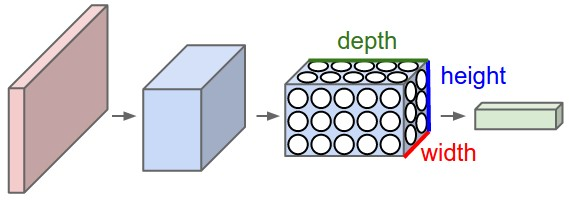
\includegraphics[width=\textwidth]{\dir/figs/convolve_data2.jpeg}
    %\caption{}
    %\label{fig.convolve_data2}
    %\end{subfigure}
    \caption[Basic Neural Network architecture]{A regular neural network, circles represent neurons. The neurons in each layer do not connect to one another but do connect to all the other neurons in the adjacent layers. Taken from \citet{karpathy_cnn1}. }
    \label{fig.convolve_data}
\end{figure}
\par
To summarise a CNN is trainable, multi-stage architecture where each stage transforms a \textit{feature map} to another through a non-linear function (\cite{lecun10}). For a generic CNN there is a convolutional layer, a pooling layer and a fully connected layer, these layers are then stacked to form a convolutional neural network.


\begin{itemize}
    
    \item The \textbf{input} layer holds the raw pixel values, for this architecture that means 256x256x3 (width x height x number of bands).
    \item The \textbf{convolutional (CONV)} layer computes the output of the neurons that are connected to local regions, each by computing a dot product between their weights and a small region they are connected to in the input volume.
    \item The \textbf{RELU} layer applies an element-wise activation function, resulting in thresholding at 0, leaving the size unchanged.
    \item The \textbf{pooling (POOL)} layer performs a downsampling along the width and height dimensions. This spatially reduces the size of the data and reduces the number of parameters to compute.
    \item The \textbf{fully connected (FC)} layer computes the class score, as this architecture is looking at a binary classification, this is either of 2 classes, the object of interest or not. 
\end{itemize}
\par
The network transforms the original image layer by layer from the original pixel values into the class scores. The CONV layer and the FC layers are functions of the activation in the input volume as well as the weights and biases of the neurons. These functions change as the weights of the network are adjusted after each training run. The RELU and POOL layers always implement a fixed function. The parameters of CONV and FC are trained with gradient descent (\cite{Bottou98,Sutskever13}) so that the class scores are consistent with the labels in the training image. In terms of our training data, the predicted class score is compared to the ground truth output to determine whether or not the network has accurately predicted the pixel value.
\par

%\section{Constructing the Convolutional Neural Network}
Before beginning data loading and processing, a generic neural network is created to process the data. This is constructed in a way that can handle any datasets with a 3-channel RGB image with an associated binary mask. The next sub-section will outline architecture needed to do this and provide an in depth discussion. 
\par
The general architecture that this network is based on is the U-Net architecture first outlined by \citet{ronneberger15}. The CNN is split into two parts, the encoder and the decoder (Figure \ref{fig.u-net_arch}). In the encoder the data is transposed and operations are performed on the data, in the decoder the data is transposed in the opposite direction while preserving the weights and biases that have been calculated by the network. Following this there is the fully connected part of the network, which is a function that compares the predicted output to that of the ground truth output before the weights are adjusted.

\begin{figure}[htbp]
    \centering
    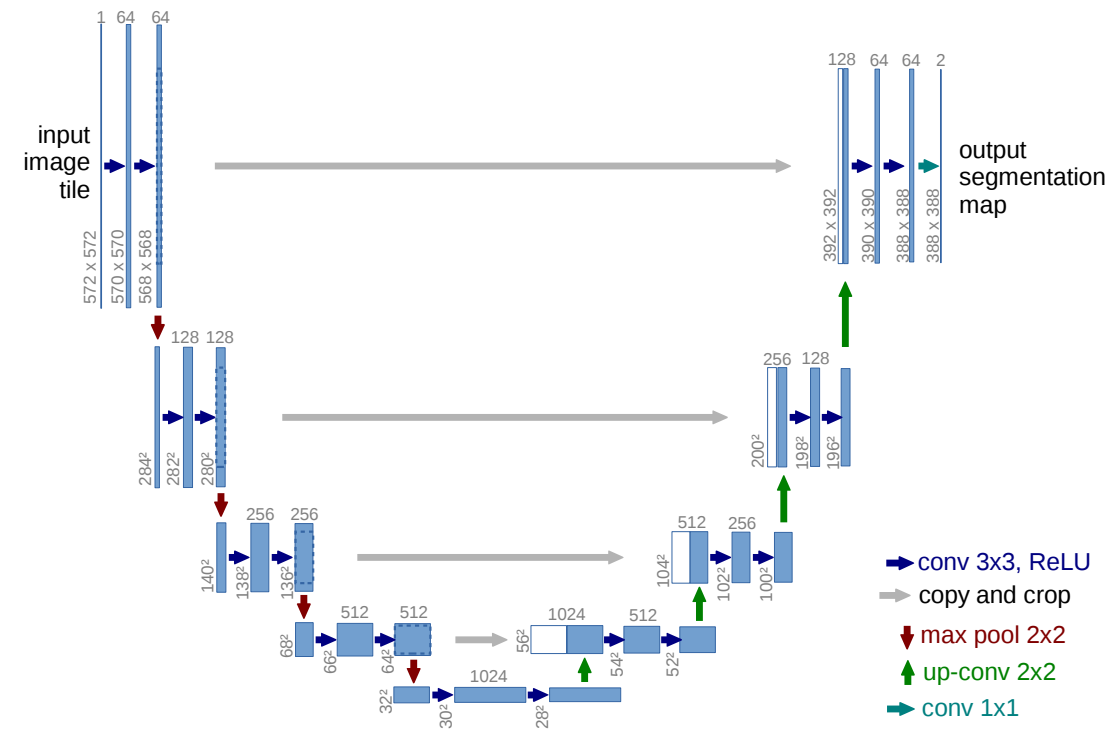
\includegraphics[width=\textwidth]{\dir/figs/unet_arch.PNG}
    \caption[Example of U-Net Architecture for a fully connected Convolutional Neural Network]{Example of U-Net Architecture for a fully connected Convolutional Neural Network. On the left the input image feeds into the encoder, on the right is the decoder before finally a prediction is made and an output segmentation map produced. Taken from \citet{ronneberger15}.}
    \label{fig.u-net_arch}
\end{figure}

\section{Convolutional Layer}
The Conv layer is the core building block for the network. It consist of a set of learnable filters, each filter is spatially small but extends through the full depth of the input. This means that for a 256x256x3 RGB image, a 4x4 filter will look at a spatially small region but at all three colour channels. Our network has been created with a filter of 4x4x3, where 4x4 represents the height and the width and 3 represents the depth of the input i.e. the number of channels or bands. This is shown in line 2 of listing \ref{lst.encoder}, where the kernel size is 4 and our in\_channel is 3. \par
%\begin{minipage}{\linewidth}
\begin{lstlisting}[language=Python, caption = {Encoder architecture, performs the convolution on the input volume at each layer in the CNN. Input is a 3D volume of depth, height and width, where the initial depth is the number of channels in the input image. The encoder convolves the data by passing a moving filter of size 4x4, with a stride of 2 and a zero padding of 1, then a batch normalisation is performed and finally an activation function is applied.}, label={lst.encoder},float,floatplacement=htbp]
class SegBlockEncoder(nn.Module):
    def __init__(self,in_channel,out_channel,kernel=4,
                stride=2,pad=1):
        super().__init__()
        self.model = nn.Sequential(
            nn.Conv2d(
                in_channel,out_channel,kernel,stride=stride,
                padding=pad,bias=False),
            nn.BatchNorm2d(out_channel),
            nn.ReLU(True)
        )

    def forward(self, x):
        y=self.model(x)
        return y
\end{lstlisting}
%\end{minipage}
As we move down through the network we pass or convolve each filter across the the width and height of the input volume, then compute a weighted sum between the entries of the filter and the input at any position. Each time the filter moves it performs a dot product between the filter and a small section of the input image. So for a 4x4x3 filter, it would be a 48 dimensional dot product plus the bias associated with the network. 
\[ w^T + b \] where $w$ is the filter.
This is adjusted when the weights and biases of the network change with each training iteration. This produces a 2D activation map that gives the response of that filter at every spatial position (Figure \ref{fig.moving_filter}). 
 
\begin{figure}[htbp]
    \centering
    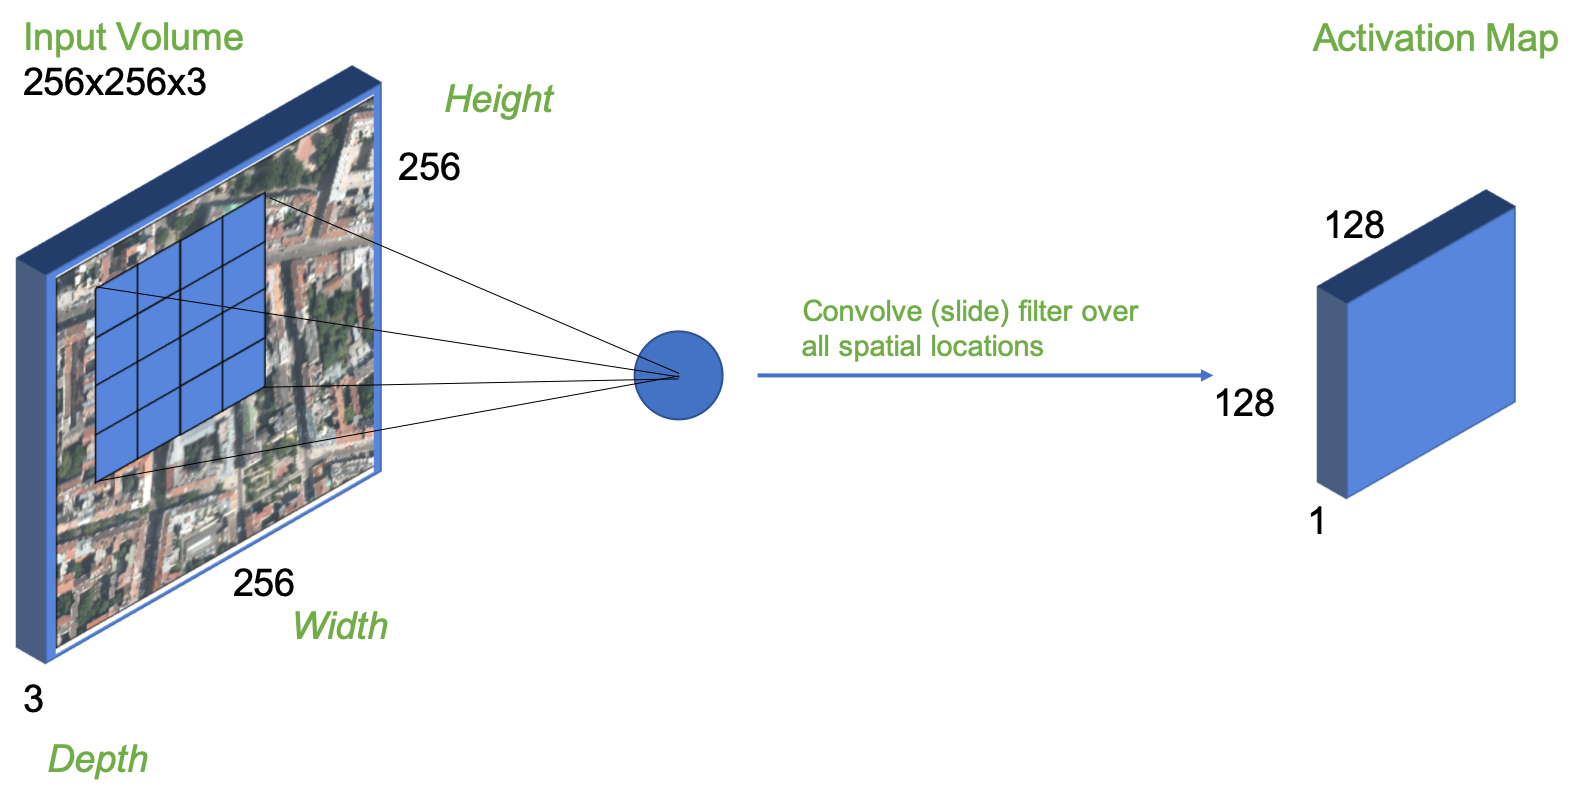
\includegraphics[width=\textwidth]{\dir/figs/moving_filter.png}
    \caption[Example of one Convolutional filter]{The Convolutional filter generates an activation map as it moves across the whole image. The stride is 2 and the padding is 1 resulting in the spatial dimensions being reduced for the output image. This is the case if their were only one filter being implemented in the Conv layer.}
    \label{fig.moving_filter}
\end{figure}
The dimensions in the output layer are controlled by the depth, stride and padding. 
\begin{enumerate}
    \item Depth of the output volume corresponds to the number of filters used to look for something in the input. For example to look for edges or colours. This is adjusted manually when fine-tuning the network in order to optimise the results.
    \item Stride for our case equals two and it defines how much the filter steps by as it moves over the image. Using two reduces the size of the output image.
    \item Padding controls the number of layers of zeroes around the input volume. 
\end{enumerate}
Intuitively the network learns filters that activate when they recognise some type of visual feature such as edges or blocks of colour in the first layer (\cite{karpathy_cnn1}). This results in an entire set of filters in each Conv layer producing separate 2D activation maps that are then stacked together along the depth axis to produce the output volume (Figure \ref{fig.conv_filter}). The filters stack together to form the new depth input that will be fed into the subsequent Conv layer. For example, if the input is 256x256x3 and we used six 4x4 filters with a stride of 2 and zero padding of 1 then the output from that layer will be 128x128x6. 

\begin{figure}[htbp]
    \centering
    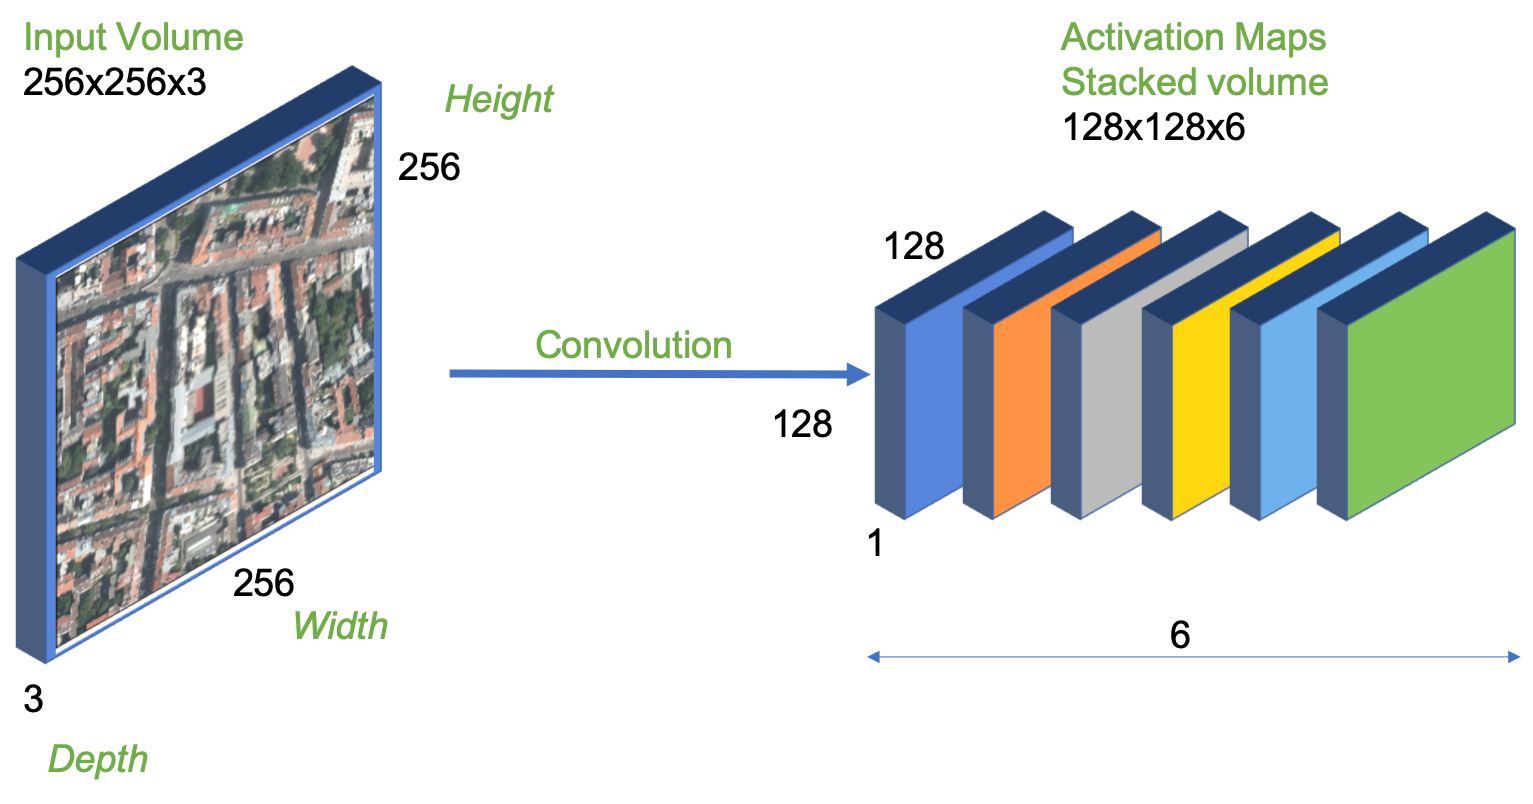
\includegraphics[width=\textwidth]{\dir/figs/stacked_activation.png}
    \caption[Example of how the Convolutional layer transforms the data using six filters]{Example of how the Convolutional layer transforms the data using six filters. Each layer on the right hand side of the image corresponds to the activation maps from a different filter. These stack together to form the input for the next layer.}
    \label{fig.conv_filter}
\end{figure}

The stride and the padding reduce the spatial dimensions and the number of filters stack together to from the depth dimension. This is then fed as the input into the next block of the network.

\section{Batch Normalisation}
Batch normalisation is a function that is used to correct for the effect of changing inputs as the network moves from layer to layer. \citet{ioffe15} were the first to recognise the affect that internal covariate shift had on deep learning. Within a single training set, the affect of internal covariate shift is not that significant but if the network is intended to predict values in another area, the effect can result in a very inaccurate model (Figure \ref{fig.cov_shift}). 
\begin{figure}[htbp]
    \centering
    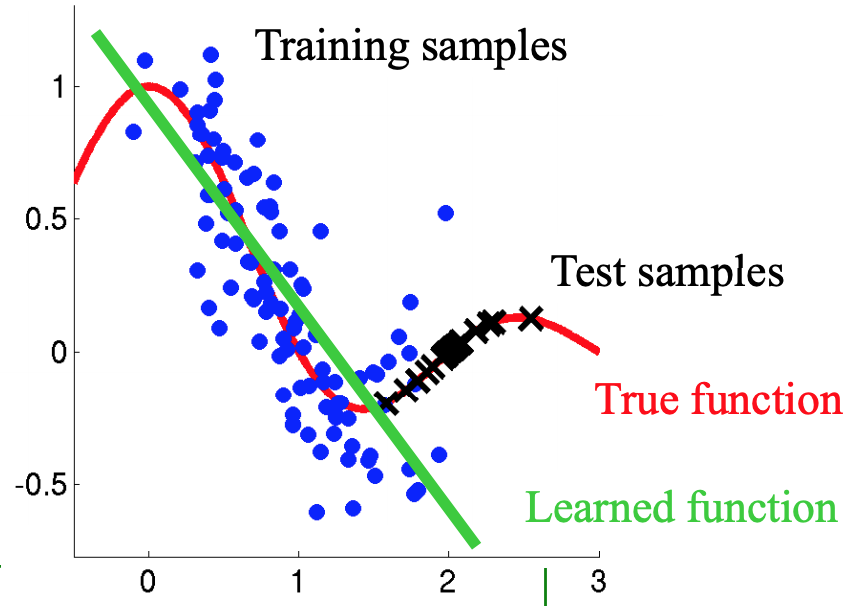
\includegraphics[width=0.5\textwidth]{\dir/figs/cov_shift.png}
    \caption[The effect of Covariate shift on a linear extrapolation]{Illustrates the effect of covariate shift on linear interpolation. Adapted from \cite{sugiyama08}.}
    \label{fig.cov_shift}
\end{figure}
Covariate shift is a result of bias in the dataset and a more in depth look and examples of the effect can be found in \citet{smola11}. By reducing the internal covariate shift, learning rates can be higher improving the time needed to achieve highly accurate models as shown in Figure \ref{fig.batchnorm}. The paper by \citet{ioffe15} claims that by using a batch normalisation function the validation error of the ImageNet classification can be dropped to below 5\% and this is better than the error expected from human raters. The normalisation occurs on the batch and is separated from the optimiser and gradient descent. Therefore the parameters are adjusted independently of the optimiser and allows for faster learning rates. \par

\section{Activation Layer}
There are many different types of activation functions that can be used with CNNs. Some of functions are better suited to different applications. ReLU(Rectified Linear Unit) is the most reliable and can be used as a good approximation for all applications. \par
Activation functions introduce non-linear properties on the network and convert an input signal to an output one. They sum the product of the inputs and their corresponding weights and apply the function to get the output and feed it as an input for the next layer. Without an activation function the output would be a linear function. These are limited in their complexity and cannot learn complex functional maps from the data. A neural network without an activation function is simply a linear regression model. Activation functions allow the user to represent non-linear arbitrary functional mappings between inputs and outputs. \par
\begin{figure}[htbp]
    \centering
    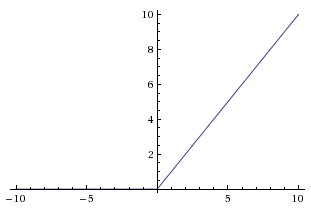
\includegraphics[width=0.5\textwidth]{\dir/figs/relu.jpeg}
    \caption{ReLu function.}
    \label{fig.relu}
\end{figure}
ReLU corrects a value to be 0 when $<$ 0 and then linear with slope of 1 when x $>$ 0. Figure \ref{fig.relu} shows the function in graphical form. \citet{krizhevsky17} shows the ReLU functions to be 6 times faster than Tanh. 
\section{Pool Layer}
It is common for CNNs to insert a pooling layer in between successive convolutional layers. This aggregates the data and reduce the parameters and computation for the network. Pooling operates independently on every depth slice (image band in the first layer, and then the stacked \textit{feature maps} subsequently) and resizes it spatially using the max function. This is analogous to raster resampling. Most commonly this process is done using a 2x2 moving filter with a stride of two that downsamples every depth slice by a factor of two. The depth dimension of the data remains unaffected by this process (Figure \ref{fig.pooling}).
\begin{figure}[htbp]
\centering
\begin{subfigure}{0.45\textwidth}
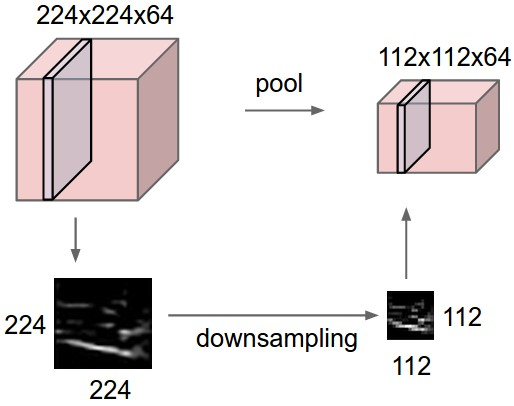
\includegraphics[width=\textwidth]{\dir/figs/pool.jpeg}
\caption{}
\label{fig.pool}
\end{subfigure}%
\qquad
\begin{subfigure}{0.45\textwidth}
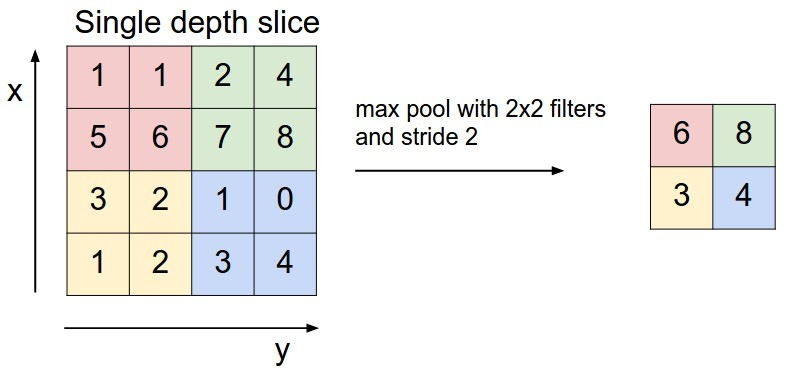
\includegraphics[width=\textwidth]{\dir/figs/maxpool.jpeg}
\caption{}
\label{fig.maxpool}
\end{subfigure}
\caption[Example of pooling and Max Pool function]{On the left we observe how the spatial dimensions of the input layer are decreased but the depth dimension remains the same. On the right we see how Max Pool assigns the greatest value to the new aggregated pixel.}
\label{fig.pooling}
\end{figure}
\par
For the CNN implemented during this project no pool layer was included. Discarding pool layers has been found to be important when training generative models and the future looks to be moving towards architectures with fewer to no pooling layers (\cite{Springenberg14}). As this thesis is aiming to produce a reusable workflow for a CNN, pool layers were not included. 

\section{Decoder}
So far we have discussed how the neural network has convolved the data and produced stacked \textit{feature maps} corresponding to what features have been identified. The next step is to backpropagate this data in order to output an image where the network has assigned a most likely class for each pixel based on the weights within the network. 
\begin{lstlisting}[language=Python, caption = {Decoder architecture, works in the opposite way to the Encoder to transpose so that dimensions match that of the ground truth for comparison.}, label={lst.decoder},float,floatplacement=htbp]
class SegBlockDecoder(nn.Module):
    def __init__(self,in_channel,out_channel, kernel=4,stride=2,pad=1):
        super().__init__()
        self.model = nn.Sequential(
            nn.ConvTranspose2d(
                in_channel,out_channel,kernel,stride=stride,padding=pad,bias=False),
            nn.BatchNorm2d(out_channel),
            nn.ReLU(True)
        )

    def forward(self, x):
        y=self.model(x)
        return y
\end{lstlisting}
The decoder is used to restore the original image size in the decoder so that the network can make a prediction about every image in the original image. This is not another convolution but rather an upsampling method that preserves the weights and biases that have been calculate within the network before a comparison between the predicted output and the ground truth output. This is called a transposed convolution, the architecture of this is shown in Listing \ref{lst.decoder}, where in line 5 we see the use of the \texttt{nn.ConvTranspose2d} function in order to deconvolve the data. This is again striving to make the CNN as simple as possible in order to make it as generative as possible (\cite{Springenberg14}).

\section{Fully Connected Layer}
The common convention for neural networks is to the last layers of the network to be fully connected layers. These are layers where all the inputs from one layer are connected to every activation unit in the next layer. FC layers accept an input from the previous layer (Pool or Conv layer in most CNNs), and output an N-dimensional vector where N is the number of classes (\cite{simard03}). This fully connected architecture works for small images, where each image belongs to one class and the network tries to identify which class that is. However, our network classifies each pixel via semantic segmentation of very large, high resolution imagery.
\par
While our network is "fully connected" it does not contain any fully connected layers as described above. Rather, the fully connected architecture is extended so that it works with very few training samples and yields more precise segmentations. The benefits of this were first demonstrated by \citet{ronneberger15}, who used this architecture very successfully for biomedical image classification.  The FC layers are replaced by the transposed convolutions in the decoder that output weights and biases in the same spatial dimensions as the input image. An example of the final architecture can be found in \citet{Richmond19a} Figure \ref{fig.unet_large}.

\section{Convolutional Neural Network}\label{sub.CNN}
In Listings \ref{lst.encoder} and \ref{lst.decoder} we have seen the architecture for the individual layers, the final stage is to tie these functions together into a final convolutional neural network as shown in Listing \ref{lst.CNN}.
\begin{lstlisting}[language=Python, caption = {A Fully connected Convolutional Neural Network. Shows how the encoder and decoder classes are arranged sequentially in order to transform the data and make a prediction on the pixel class.}, label={lst.CNN},float,floatplacement=htbp]
class Net(nn.Module):
    def __init__(self,cr = 2):
        self.cr = cr
        super(Net,self).__init__()
        self.encoder = nn.Sequential(
            SegBlockEncoder(in_channel=3,out_channel=self.cr),
            SegBlockEncoder(in_channel=self.cr,out_channel=self.cr*2),
            SegBlockEncoder(in_channel=self.cr*2,out_channel=self.cr*4),
            SegBlockEncoder(in_channel=self.cr*4,out_channel=self.cr*8),
            SegBlockEncoder(in_channel=self.cr*8,out_channel=self.cr*16)
        )
        self.decoder = nn.Sequential(
            SegBlockDecoder(in_channel=self.cr*16, out_channel=self.cr*8),
            SegBlockDecoder(in_channel=self.cr*8, out_channel=self.cr*4),
            SegBlockDecoder(in_channel=self.cr*4, out_channel=self.cr*2),
            SegBlockDecoder(in_channel=self.cr*2,out_channel=self.cr),
            SegBlockDecoder(in_channel=self.cr, out_channel= 2))
        
        self.output = nn.Softmax(dim = 1)
        
    def forward(self,x):
        x1 = self.encoder(x)
        x2 = self.decoder(x1)
        y = self.output(x2)
        return y
\end{lstlisting}
For this architecture there are five layers for the forward pass, and five layers for the mirrored backward pass. In Listing \ref{lst.CNN} line 2 cr corresponds to the number of filters in the convolutional layer. This is a hyperparameter and needs to be adjusted in order to fine tune the model to optimise the results. The softmax function on line 21 is a binary linear regression classifier for multiple classes. It allows the user to compute the probability of a pixel belonging to one class or another and forms the output of the CNN.
\subsection{Softmax Classifier}\label{sec.softmax}
The final layer of the CNN outputs a multidimensional array with the raw scores for each pixel. As our model is a binary classification problem, the score corresponds to how likely the pixel belongs to one class or the other. The vector is then input into the softmax classifier, which outputs the probability scores that sum to 1. For each pixel, the softmax classifier takes the exponent of the raw score for each class and divides it by the sum of the exponents of all raw class scores. As shown below:
\[S_{y_i} = \frac{e^{y_i}}{\sum_j e^{y_j}}\]



